\documentclass[aspectratio=169,10pt]{beamer}
\usetheme{default}\usecolortheme{default}
\usepackage[T1]{fontenc}\usepackage[utf8]{inputenc}
\usepackage{lmodern,microtype,booktabs,tabularx,graphicx,amsmath}
\usepackage{xcolor}
\definecolor{ink}{HTML}{2F3437}\definecolor{muted}{HTML}{6B7378}
\definecolor{faint}{HTML}{9AA3AB}\definecolor{blue}{HTML}{2A78D6}
\definecolor{orange}{HTML}{EB6834}\definecolor{aqua}{HTML}{1BAF7A}
\definecolor{paper}{HTML}{FCFCFB}
\setbeamercolor{background canvas}{bg=paper}
\setbeamercolor{frametitle}{fg=ink,bg=paper}
\setbeamercolor{normal text}{fg=ink}
\setbeamercolor{structure}{fg=blue}
\setbeamerfont{frametitle}{series=\bfseries,size=\large}
\setbeamertemplate{navigation symbols}{}
\setbeamertemplate{itemize items}[circle]
\setbeamertemplate{footline}{\hfill\tiny\color{faint}\insertframenumber/10\hspace{4mm}\vspace{2mm}}
\setlength{\parskip}{3pt}
\newcommand{\lead}[1]{{\color{blue}\bfseries #1}}
\newcommand{\aside}[1]{\vspace{2mm}\par{\footnotesize\color{muted}#1}}
\newcommand{\keymsg}[1]{\vspace{2mm}\begin{beamercolorbox}[wd=\textwidth,sep=2mm]{}\color{orange}\bfseries #1\end{beamercolorbox}}
\graphicspath{{../figures/}}
\begin{document}

\begin{frame}[plain]
\vspace{14mm}
{\LARGE\bfseries\color{ink} Context-Dependent Selection\\[1mm] of Urban Routing Policies}\\[6mm]
{\large\color{muted} Methodological redesign --- proposal for discussion}\\[10mm]
{\footnotesize\color{faint} Version 2 design. No V2 experiment has been run; all V2 quantities are
specifications or hypotheses.}
\end{frame}

\begin{frame}{1 \quad The problem}
A navigation or traffic operator selects \emph{one} routing strategy for an operating episode.
Different strategies optimise different objectives, so they fail under different traffic conditions.
\vspace{3mm}
\begin{center}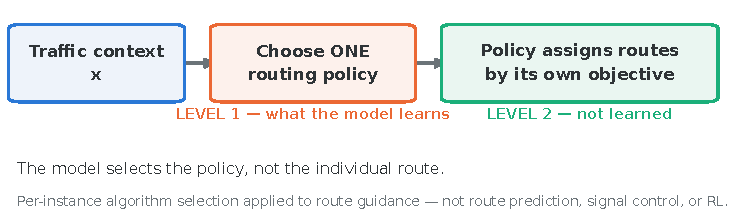
\includegraphics[width=.86\textwidth]{v2_two_levels.pdf}\end{center}
\keymsg{Can we determine, before deployment, which routing policy is appropriate for the current traffic context?}
\end{frame}

\begin{frame}{2 \quad Why the current formulation needs redesign}
\begin{enumerate}
\item \lead{Weak policy complementarity.} The policies largely shared one failure mode, so the
      winner map reduced to a single demand variable.
\item \lead{Highly correlated decision criteria.} Travel time and CO$_2$ moved together; the
      multi-criteria layer changed no decision.
\item \lead{The adaptive model was close to a simple demand rule.} One split captured most of the
      available decision value.
\end{enumerate}
\keymsg{The redesigned study will first test whether meaningful policy complementarity exists.}
\aside{Version 1 answered its question honestly, and the answer was narrow. Complementarity is now a
hypothesis under test --- not a design assumption.}
\end{frame}

\begin{frame}{3 \quad What exactly are we selecting?}
\begin{center}
\begin{tabular}{@{}ll@{}}
\lead{Level 1} & context $\longrightarrow$ routing policy \quad {\color{orange}\itshape the model learns this}\\[1mm]
\lead{Level 2} & policy $\longrightarrow$ individual routes \quad {\color{muted}\itshape the policy's own objective}\\
\end{tabular}
\end{center}
\vspace{3mm}
\begin{center}
Provisional portfolio:\\[1.5mm]
\textbf{static / shortest} \quad\textbf{reactive travel time}\\[1mm]
\textbf{capacity-aware load balancing} \quad\textbf{reliability-aware}
\end{center}
\vspace{4mm}

\aside{Per-instance algorithm selection applied to route guidance, with the simulator as the
performance oracle. Not route prediction, not signal control, not reinforcement learning.}
\end{frame}

\begin{frame}{4 \quad Different policies have different failure modes}
\scriptsize
\begin{tabularx}{\textwidth}{@{}lXXX@{}}
\toprule
\textbf{Policy} & \textbf{Main strength} & \textbf{Main weakness} & \textbf{Triggering condition}\\
\midrule
Static / shortest & simple, efficient & overloads its own preferred route & demand approaches shortest-corridor capacity\\[1mm]
Reactive travel time & responds to congestion & information lag, \textbf{herding}, oscillation & high penetration; lag long vs trip time; abrupt events\\[1mm]
Capacity-aware & balances load across alternatives & spreads traffic that needed no spreading & light demand; one dominant path\\[1mm]
Reliability-aware & avoids highly variable routes & detour premium when conditions are stable & stable conditions; noisy variance estimate\\
\bottomrule
\end{tabularx}
\keymsg{A portfolio is selectable only if its members fail for different reasons.}
\end{frame}

\begin{frame}{5 \quad What creates the different regimes?}
\begin{center}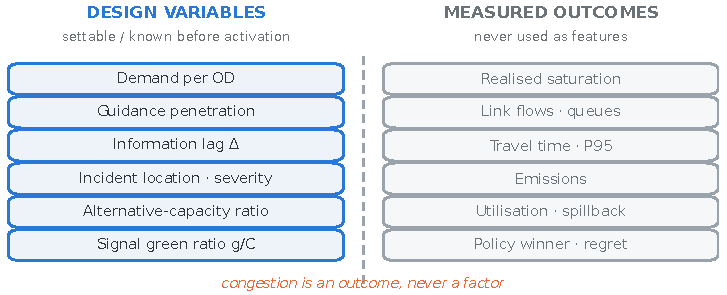
\includegraphics[width=.80\textwidth]{v2_factors.pdf}\end{center}
\aside{Penetration and incidents are the two factors the previous design could not vary. Without
penetration there is no herding; without incidents there is no travel-time variance --- so two of
the four policies would have nothing to be good at.}
\end{frame}

\begin{frame}{6 \quad Decision framework: avoiding arbitrary weights}
The additive $0.5/0.5$ weighting is \lead{removed as the primary method}.
\vspace{2mm}
\begin{enumerate}
\item \lead{Pareto screening} --- remove dominated policies. No weights required.
\item \lead{System-level mean journey time} over all traffic --- ranks the survivors.
\item \lead{Preference sensitivity} --- reported only where a genuine conflict survives step 1.
\end{enumerate}
\vspace{1mm}
If a scalar is needed: generalised cost from \emph{published} VOT / VOR / carbon values, with a
sensitivity range.
\keymsg{We do not invent weights merely to create a winner.}
\aside{The system-level objective also charges a policy for its effect on background traffic.}
\end{frame}

\begin{frame}{7 \quad What does the ML actually learn?}
\begin{center}
context $\rightarrow$ mechanistic features $\rightarrow$ \textbf{advantage model} $\rightarrow$
per-policy advantage $\rightarrow$ ranking $\rightarrow$ recommended policy
\end{center}
\vspace{2mm}
The model predicts \lead{advantage relative to a baseline}
\[ \Delta_a(x) \;=\; C_{\mathrm{SBS}}(x) - C_a(x) \]
not raw travel time --- centring the target on zero at the decision boundary.
\vspace{1mm}
\aside{Strong tabular ML (gradient-boosted trees), not a deep model: low-dimensional,
interaction-heavy, context-level instances. A graph network or an RL formulation would be
sophistication without a matching problem structure.}
\end{frame}

\begin{frame}{8 \quad Robustness: when should we trust the selector?}
\begin{center}
new context $\rightarrow$ \textcolor{aqua}{\bfseries support gate} $\rightarrow$
\textcolor{aqua}{\bfseries confidence gate} $\rightarrow$ \textbf{ACT} \quad or \quad
\textbf{ABSTAIN} $\rightarrow$ fixed policy
\end{center}
\vspace{2mm}
Shift types tested \emph{separately}: interpolation $\cdot$ extrapolation $\cdot$ unseen incident
$\cdot$ unseen OD $\cdot$ unseen topology.
\keymsg{The selector is allowed to say: I do not know.}
\aside{Motivated by our own evidence: holding out a whole demand level made the previous selector
\emph{worse than the fixed policy it replaced}. Caveat on the record --- conformal prediction
guarantees coverage only under exchangeability, so it is a calibrated gate in-distribution and a
heuristic outside it. The \emph{support} gate is what addresses extrapolation.}
\end{frame}

\begin{frame}{9 \quad Evaluation: does ML really add decision value?}
\begin{center}
best fixed $\rightarrow$ \textbf{mechanistic rule} $\rightarrow$ standard ML $\rightarrow$
GBDT $\rightarrow$ selective GBDT\\[1mm]
{\footnotesize\color{muted} reference: cross-fitted hindsight best policy --- retrospective, not deployable}
\end{center}
\vspace{2mm}
Primary metrics: regret $\cdot$ closed VBS--SBS gap $\cdot$ CVaR$_{90}$ regret $\cdot$ OOD risk
$\cdot$ non-inferiority.
\keymsg{Critical test: does the model beat the strong mechanistic rule?}
\aside{Beating the best fixed policy is too low a bar. If the rule wins, the finding is that the
decision is mechanistically simple --- and we report that.}
\end{frame}

\begin{frame}{10 \quad Expected contribution}
\lead{Hypotheses, not results:}
\begin{enumerate}\itemsep1mm
\item Routing policies will show complementary strengths across operating regimes.
\item The strongest policy will depend on traffic, network \emph{and information} conditions ---
      not demand alone.
\item A mechanism-informed selector will capture useful policy-selection structure.
\item Uncertainty and abstention will reduce harmful decisions under distribution shift.
\item The study will identify when adaptive selection is genuinely useful and when a fixed strategy
      is sufficient.
\end{enumerate}
\vspace{2mm}
{\color{ink} We aim to characterise the operating regions of established routing policies and develop
a context-aware, uncertainty-aware method for selecting among them.}
\keymsg{Decision required: portfolio $\cdot$ scenario factors $\cdot$ decision objective $\cdot$ ML architecture}
\end{frame}

\begin{frame}[plain]{Appendix --- full architecture}
\begin{center}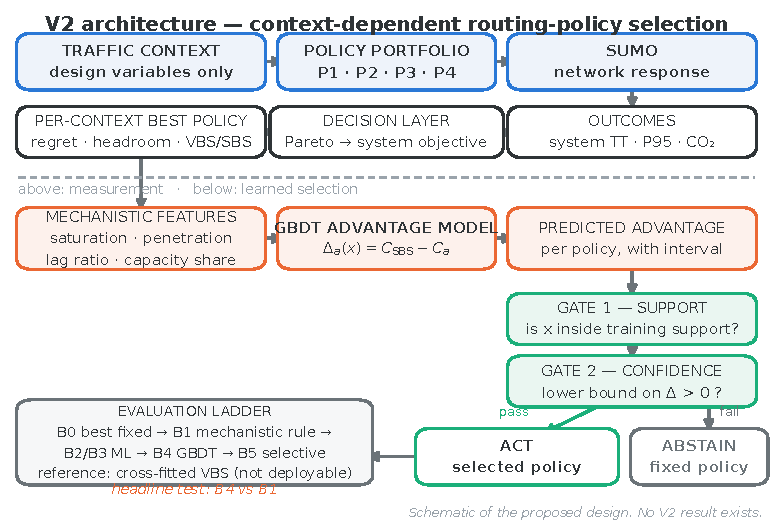
\includegraphics[height=.80\textheight]{v2_architecture.pdf}\end{center}
\end{frame}

\end{document}
